\documentclass{article}
\usepackage[paperwidth=18.5in,paperheight=8.25in,margin=0in]{geometry}
\usepackage{graphicx}
%\usepackage[showboxes,absolute]{textpos}
\usepackage[absolute]{textpos}
\usepackage{bold-extra}
\usepackage{tikz}
\usepackage{color}
\usepackage{tgbonum}
\usepackage{rotating}
\setlength{\TPHorizModule}{1in}
\setlength{\TPVertModule}{1in}
\definecolor{AuthorColor}{rgb}{1,1,1}%{0.2156863 0.3882353 0.5882353}
\definecolor{TitleColor}{rgb}{1,1,1}%{0,0,0}
\definecolor{RColor}{rgb}{0.2156863 0.3882353 0.5882353}%{0.5725490,0.7098039,0.8588235}%{0.3372549,0.4392157,0.1843137}%{0.2529412,0.5,0.2392157}


\begin{document}

{\fontfamily{phv}\selectfont




%%%% Back Cover Lightener
%\begin{textblock}{6.188}(-0.2,0)
%\noindent\begin{tikzpicture}
%\fill [white,opacity=.2] (0in,-8.25in) rectangle (6.188in,0in);
%\end{tikzpicture}
%\end{textblock}

%%%% Back Cover Contents


\begin{textblock}{5}(3.4,.8)
\raggedright


\noindent\textsc{\bfseries{The Five College Guide to Statistics with
    R}} provides instructors with a head start in using R to teach
statistics and data science.  This guide was assembled from the
author's decade-long experience running workshops for the statistics education
community.  The title refers to the five-college consortium ---
Amherst College, Mount Holyoke College, Smith College, Hampshire
College and the University of Massachusetts Amherst --- which has an
ongoing set of workshops to help instructors get started using R as an
instructional tool.

\medskip

\noindent Other books in the Project MOSAIC series include:
\begin{itemize}
\item \textsc{Start Modeling with R}
\item \textsc{Start Teaching with R}
\item \textsc{Start R in Calculus}
\end{itemize}

\raggedright
\noindent \noindent {\bf Nicholas Horton}, {\bf Randall Pruim}, and {\bf
Daniel Kaplan} teach statistics, mathematics, and computation at
Amherst College, Calvin College, and Macalester College
respectively.  They are co-PIs on the National Science Foundation
support Project MOSAIC (NSF DUE-0920350).

\medskip

\centerline{\begin{tabular}{ccc}
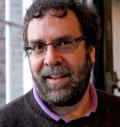
\includegraphics[height=1in]{../../CoverImages/horton.jpg} & 
\includegraphics[height=1in]{../../CoverImages/pruim.jpg} & 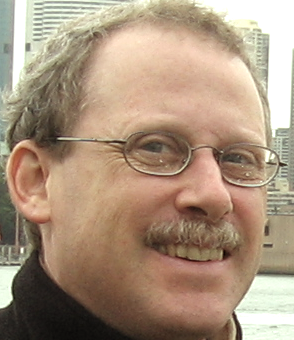
\includegraphics[height=1in]{../../CoverImages/kaplan.png}\\
{\sc Horton} & {\sc Pruim} & {\sc Kaplan}\\
\end{tabular}}

\medskip

\noindent {\bf Other books by the authors:}\\
{\em Using R for Data Management, Statistical Analysis and Graphics} (NJH \& KK)\\
{\em Foundations and Applications of Statistics: An Introduction Using
  R } (RJP), {\em Gems of Theoretical Computer Science} (US \& RJP),
{\em Understanding Nonlinear Dynamics} (DTK), {\em Statistical Modeling: A Fresh Approach} (DTK), {\em Start R in Calculus} (DTK)

\medskip

\noindent{\small Cover photo by Maya Hanna}
\end{textblock} 

\begin{textblock}{4}(3.3,.5)
\noindent\begin{tikzpicture}
\fill [white,opacity=.5] (0in,-6.1in) rectangle (5.4in,0in);
\end{tikzpicture}
\end{textblock}


%%%% Front Cover Lightener
\begin{textblock}{6.188}(8.8,0)
\noindent\begin{tikzpicture}
\fill [white,opacity=.3] (0in,-8.25in) rectangle (6.581in,0in);
\end{tikzpicture}
\end{textblock}

%%%% Title

\begin{textblock}{5.2}(9.1,1.8)
\noindent{%
\hbox{\parbox{4.5in}{\noindent\raggedleft{\textsc{\bfseries{%
\fontsize{28pt}{60pt}\selectfont\textcolor{TitleColor}{%
\hfill A Compendium  of\newline \hspace{0pt} \newline\hspace{0pt}{\tiny .}\hfill
Commands to Teach%
\newline \hspace{0pt} \newline\hfill Statistics with }}}}}\bfseries{{\fontsize{150pt}{60pt}\selectfont\textcolor{RColor}{\raisebox{-.75in}{R}}}}}}
\end{textblock}

\begin{textblock}{4.5}(10,5.5)

\noindent{\textsc{\bfseries{\fontsize{22pt}{60pt}\selectfont
     \textcolor{AuthorColor}{Nicholas J. Horton\\\\Randall
       Pruim\\\\Daniel T. Kaplan}}}}
\end{textblock}

% Spine
\begin{textblock}{0.204}(9.19,0)

\vspace*{.4in}

\noindent\hspace{-.2in}\rotatebox{270}{\large\bf
  \textcolor{yellow}{Compendium of Commands to Teach with
    R}\hspace{.3in}Horton, Pruim, Kaplan
  \hspace{.3in}{\textcolor{yellow}{\sf Project MOSAIC}}\hspace*{.25in}\raisebox{-1.3mm}{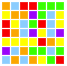
\includegraphics[width=0.21in]{../../CoverImages/mosaic-square.png}}}


\end{textblock}

%%% Mosaic Logo
\begin{textblock}{1.5}(3.6,6.65)
\noindent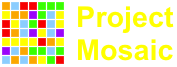
\includegraphics[width=1.5in]{../../CoverImages/mosaic-logo-small.png}
\medskip
\noindent \rule{2pt}{0pt}
\includegraphics[width=1.425in]{../../CoverImages/RStudio.png}
\end{textblock}

%% Back Flap

\begin{textblock}{3}(-.1,.15)
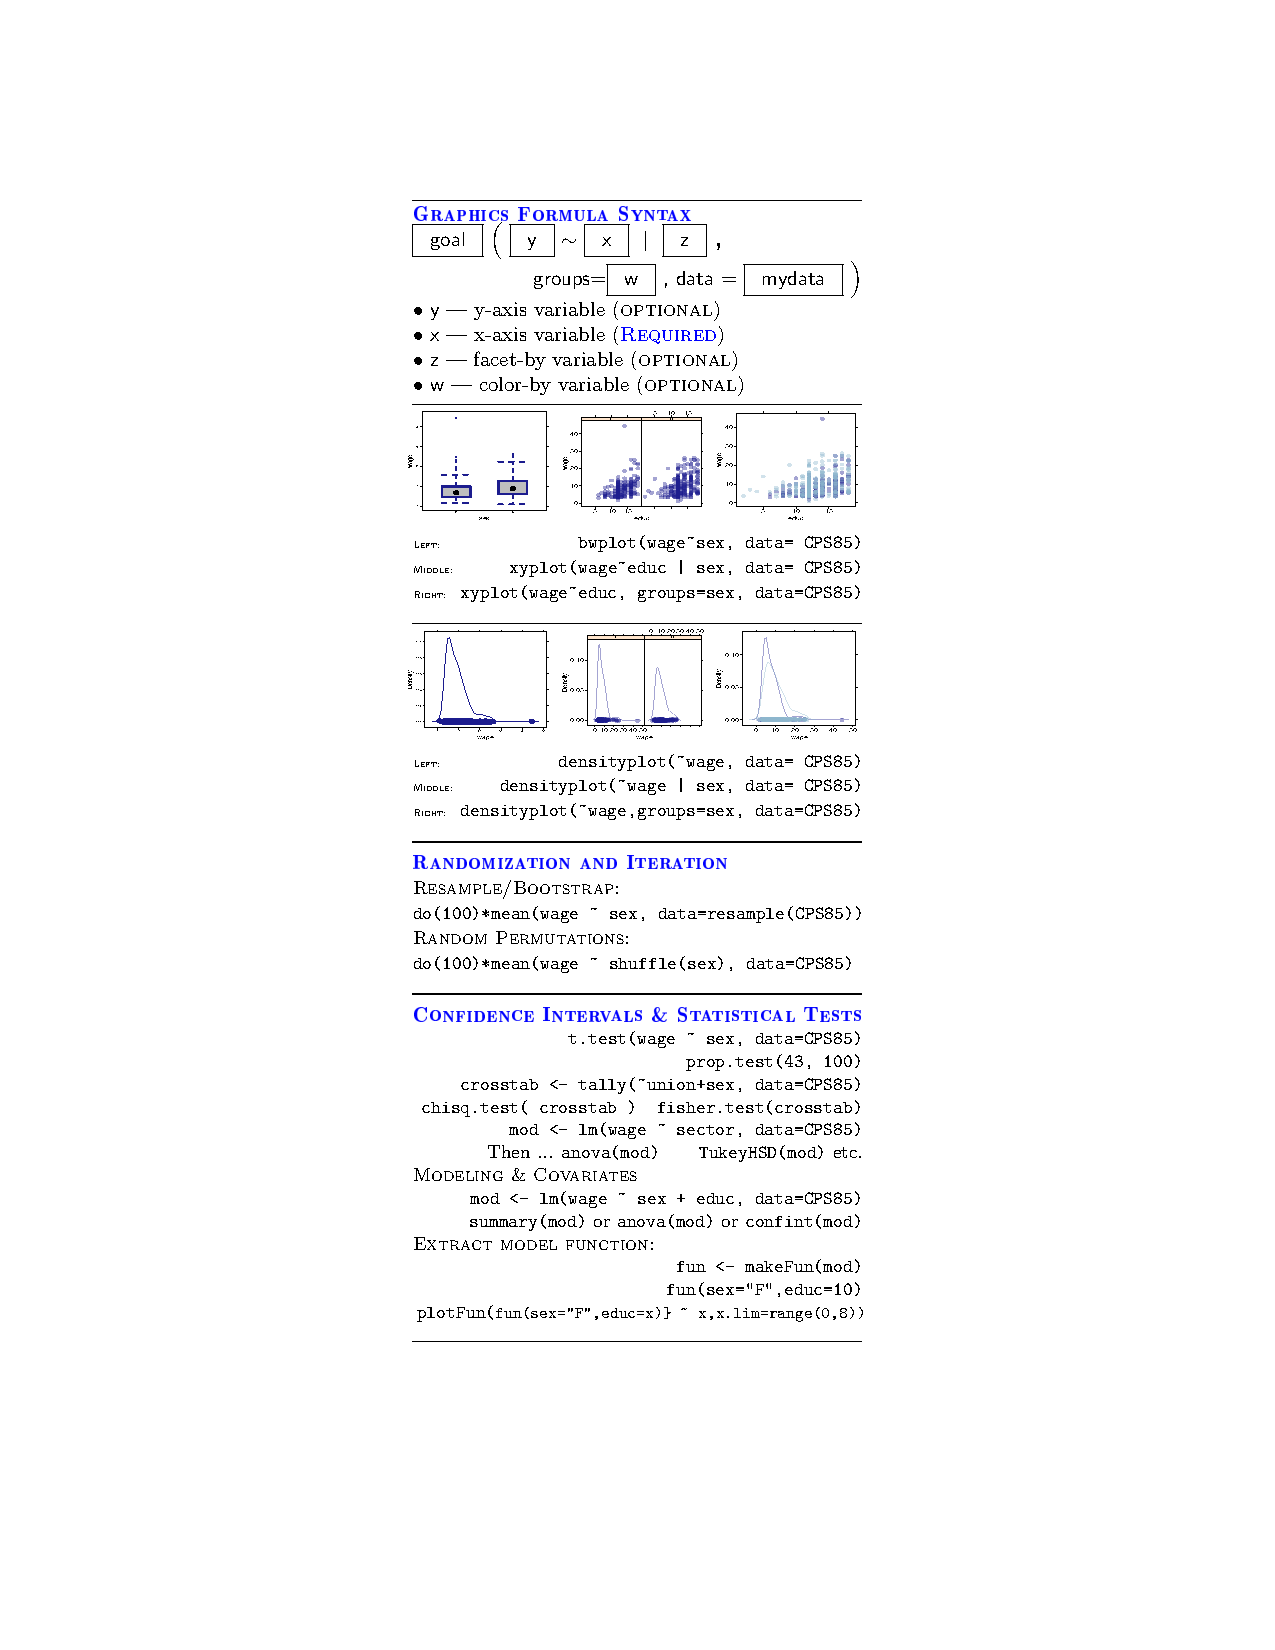
\includegraphics[width=2.9in]{backflap.pdf}
\end{textblock}

\begin{textblock}{3}(0,0)
\noindent\begin{tikzpicture}
\fill [white,opacity=.5] (0in,0in) rectangle (3in,8.4in);
\end{tikzpicture}
\end{textblock}

% Front Flap

\begin{textblock}{3}(15.3,.15)
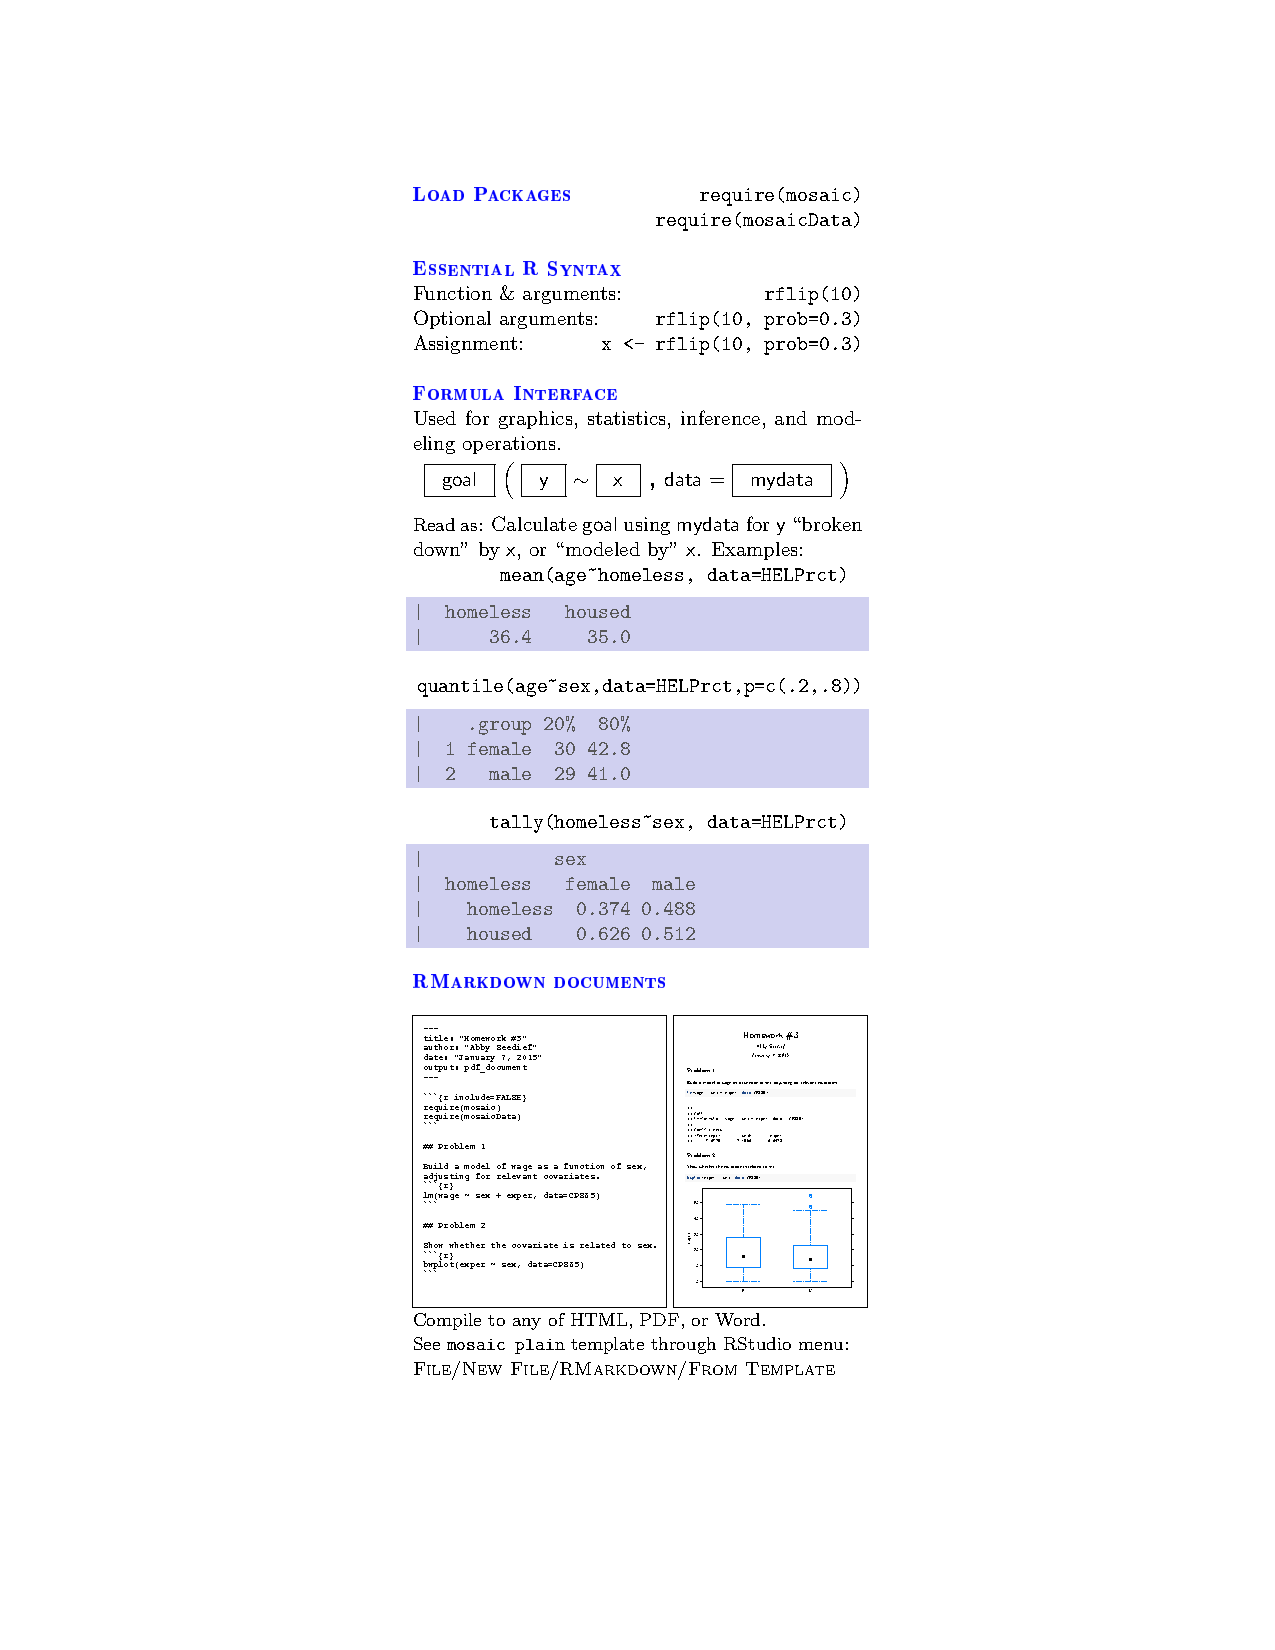
\includegraphics[width=2.9in]{frontflap.pdf}
\end{textblock}

\begin{textblock}{3}(15.5,0)
\noindent\begin{tikzpicture}
\fill [white,opacity=.5] (0in,0in) rectangle (3in,8.4in);
\end{tikzpicture}
\end{textblock}

%%% ISBN 978-0-9839658-8-6
\begin{textblock}{1.65}(6.6,6.85)   % Same as above
\noindent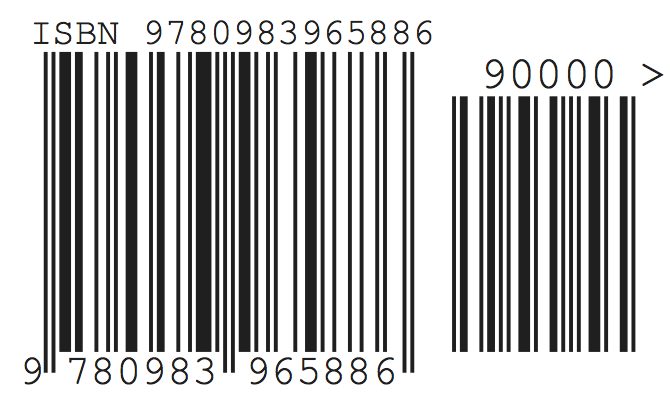
\includegraphics[width=1.75in]{../../CoverImages/ISBN-8-6.png}
\end{textblock}
\begin{textblock}{1.65}(6.6,6.85)
\noindent\begin{tikzpicture}
\fill [white,opacity=.6] (-1.75in,-1in) rectangle (0in,0in);
\end{tikzpicture}
\end{textblock}



% Front Photo

\begin{textblock}{6.125}(8.9,0)
\noindent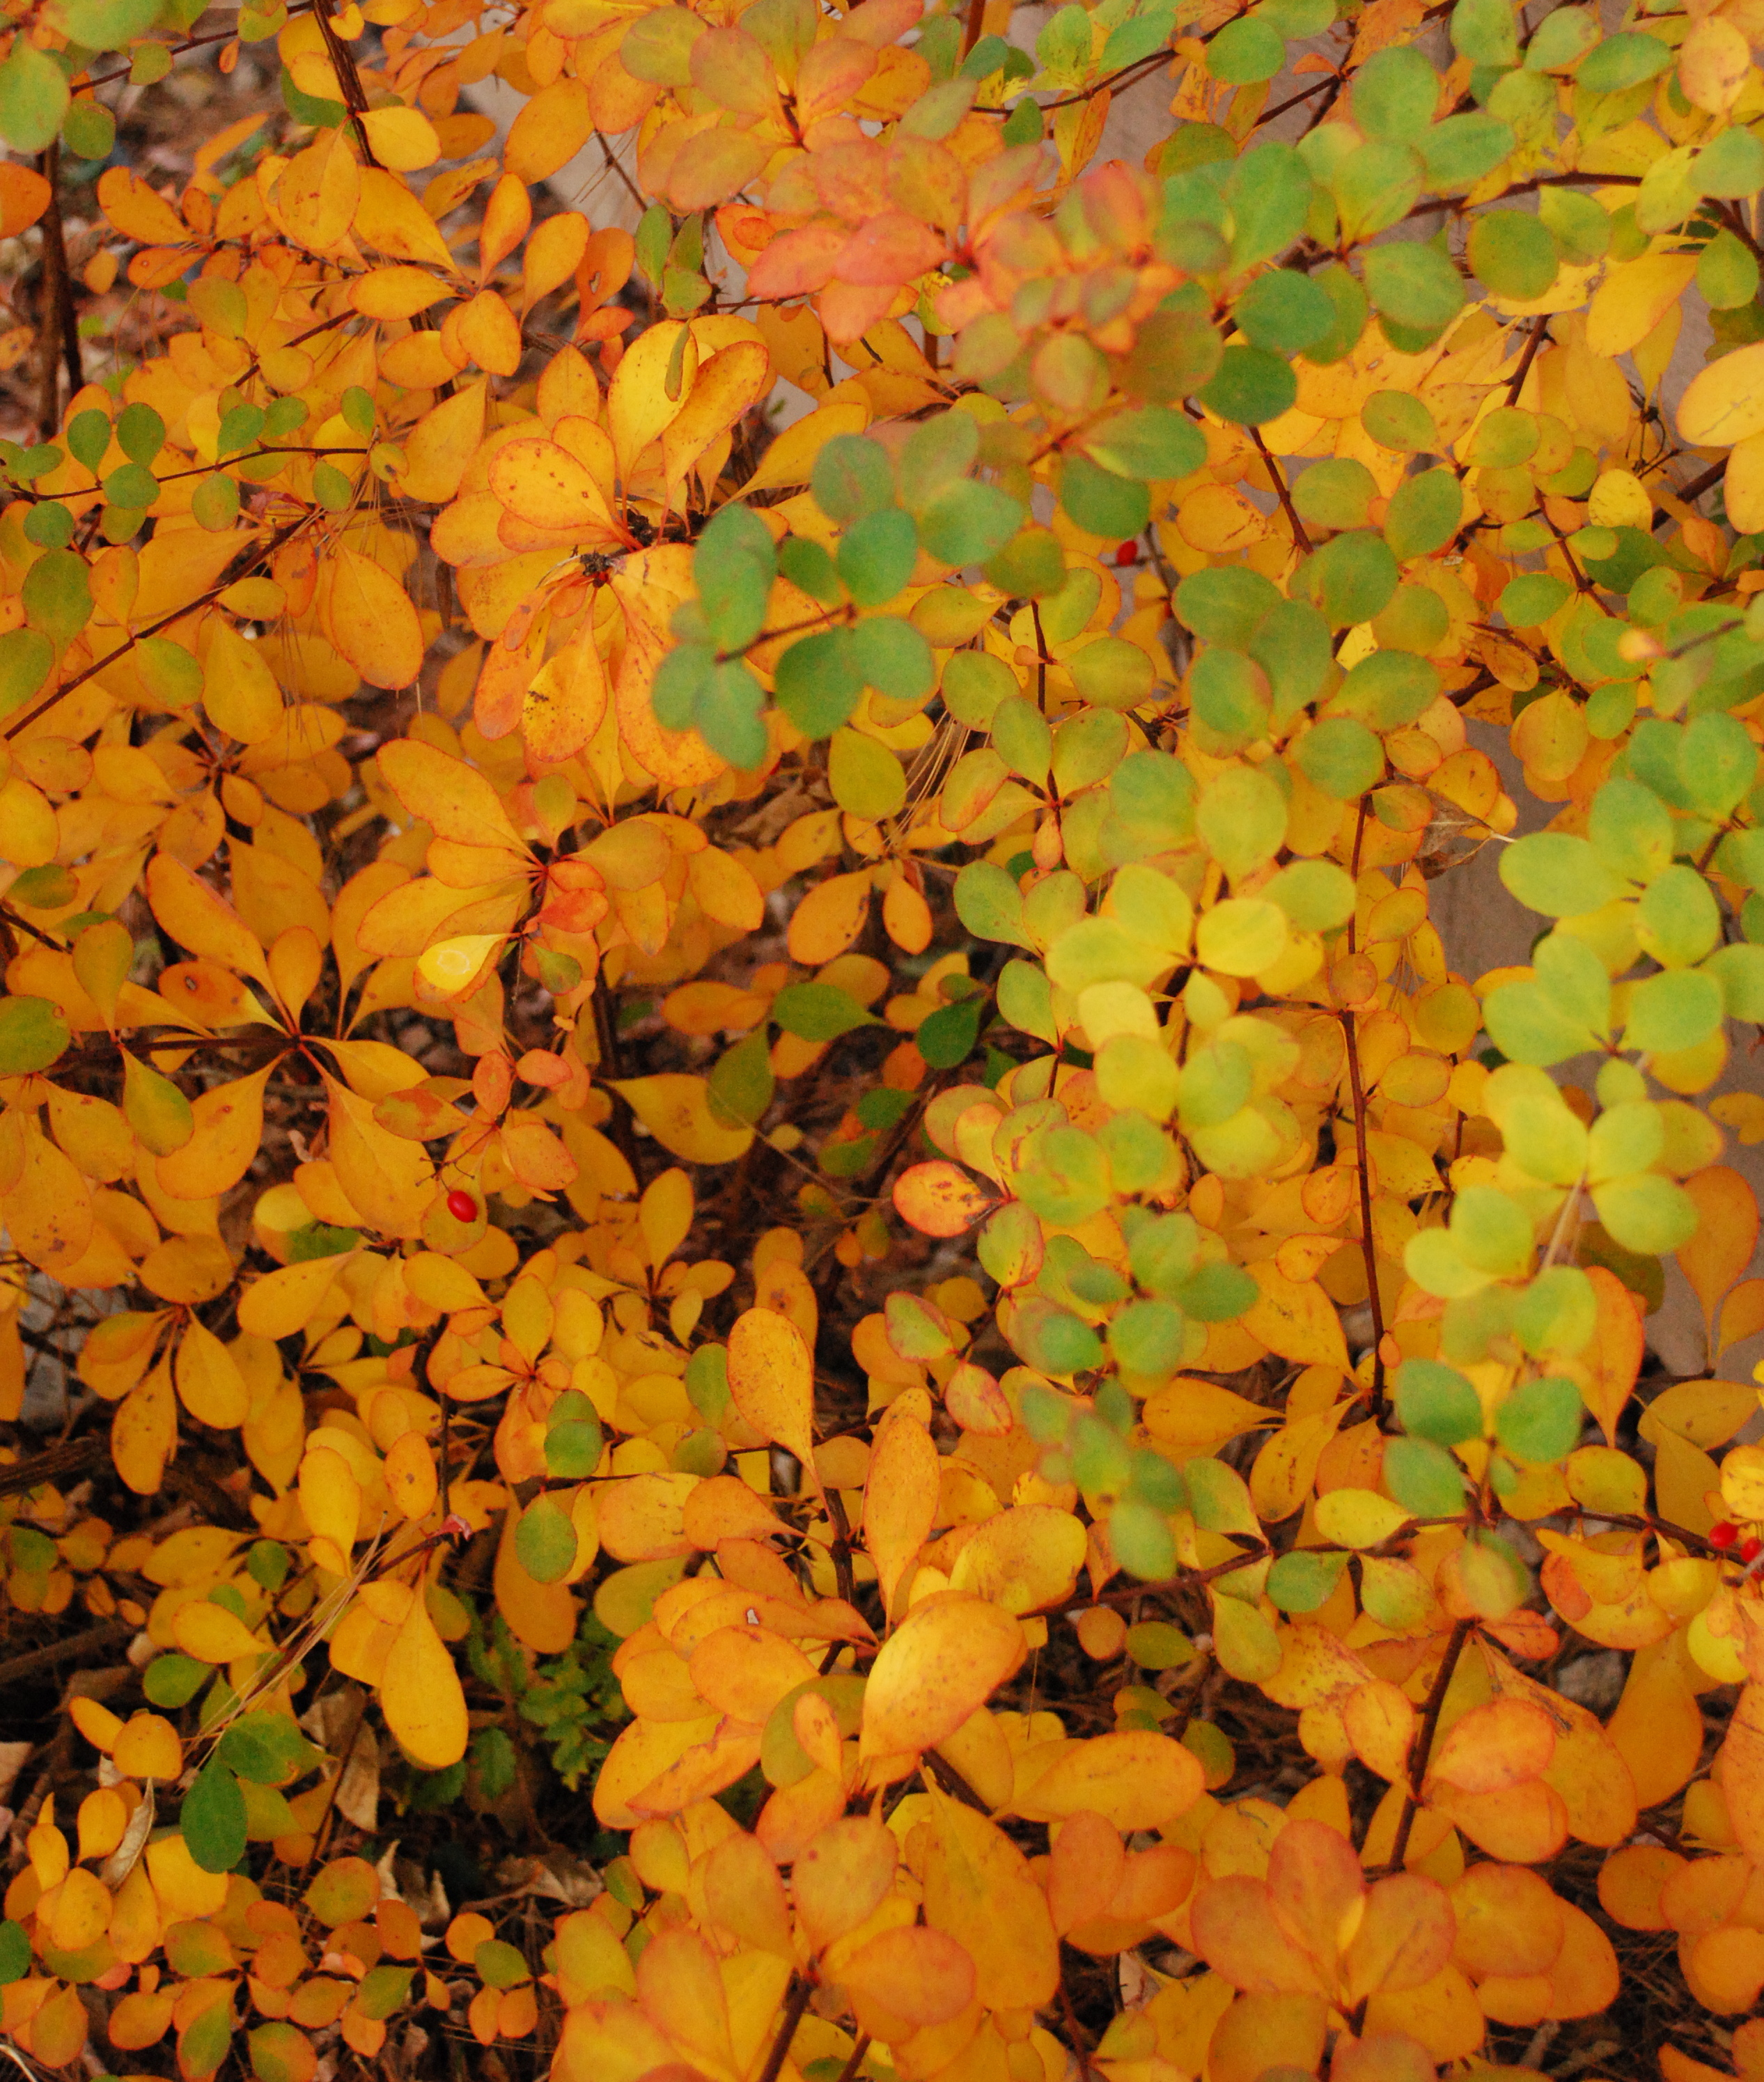
\includegraphics[angle=90,height=8.25in,width=9.881in]{../../CoverImages/FrontMain.jpg}
\end{textblock}

% Back Photo

\begin{textblock}{6.125}(-.2,0)
\noindent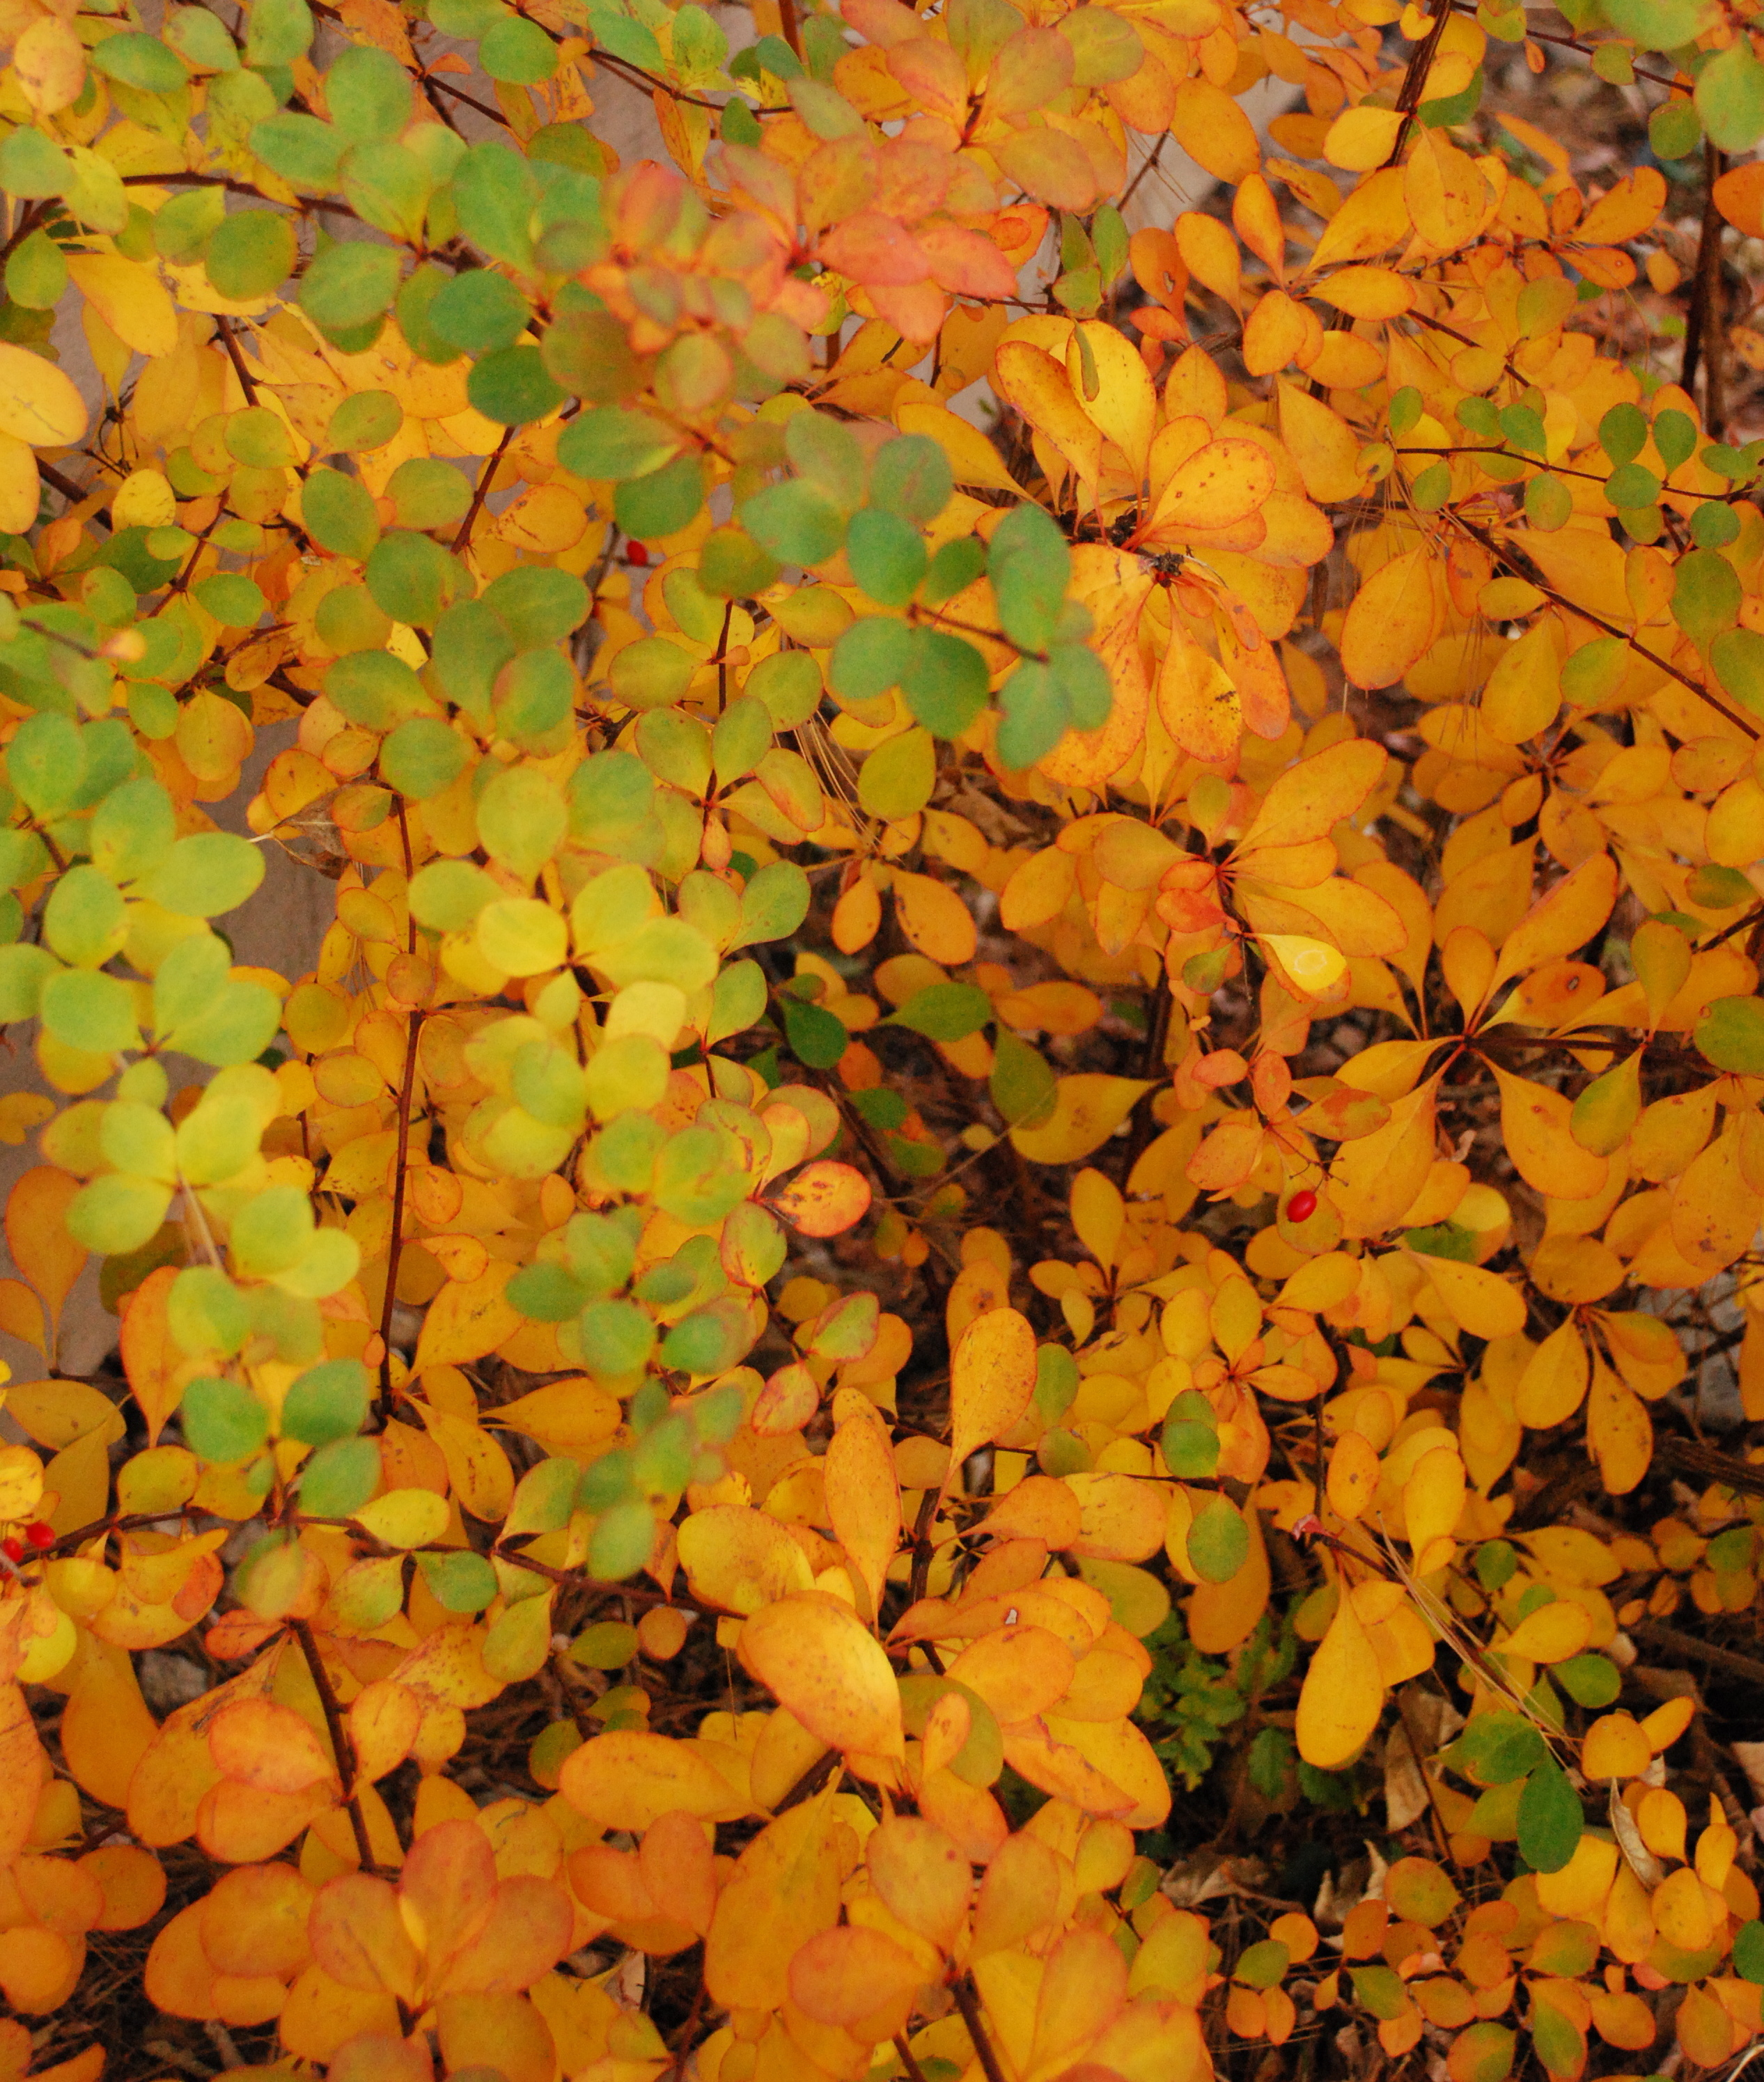
\includegraphics[angle=90,height=8.25in,width=9.881in]{../../CoverImages/BackMain.jpg}
\end{textblock}


\end{document}

